\documentclass[11pt,a4paper]{article}

\usepackage[a4paper,margin=1in]{geometry}
\usepackage{graphicx}
\usepackage{booktabs}
\usepackage{float}
\usepackage{hyperref}
\usepackage{xcolor}
\usepackage{listings}
\usepackage{enumitem}
\usepackage{fancyhdr}

\hypersetup{colorlinks=true,linkcolor=blue,urlcolor=blue}

\pagestyle{fancy}
\setlength{\headheight}{14pt}
\fancyhf{}
\lhead{Computer Networks Laboratory}
\rhead{Assignment 2}
\cfoot{\thepage}

\lstdefinestyle{cstyle}{
  language=C,
  basicstyle=\ttfamily\small,
  numbers=left,
  numberstyle=\tiny,
  frame=single,
  breaklines=true,
  showstringspaces=false,
  keywordstyle=\color{blue},
  commentstyle=\color{gray},
  stringstyle=\color{purple}
}
\lstset{style=cstyle}

\setlength{\parskip}{0.5em}
\setlength{\parindent}{0pt}

\begin{document}

\begin{center}
{\LARGE \textbf{Assignment 2: Multi-Client Chat Application using TCP and UDP Sockets}}\\[4mm]
Simiyon Vinscent Samuel L\\
Register Number: 3122247001062\\
Submission Date: August 17, 2026\\
GitHub Repository: \url{https://github.com/blackscythe123/PCN-assign}
\end{center}

\vspace{2mm}
\hrule
\vspace{4mm}

\section*{Aim}
To build a small client-server system in C that lets a student look up their academic
record by roll number -- once over TCP, returning the full profile, and once over UDP,
returning just enough to confirm the record exists -- both reading from the same
\texttt{students.csv}. The point of the exercise is really to feel the practical
difference between a connection-oriented, reliable transport and a connectionless one for
the same basic lookup task, not the lookup itself.

\section*{Reading the Student Data}
Both servers keep this deliberately simple: on startup they open \texttt{students.csv},
skip the header line, and split each remaining line on commas straight into an array of
\texttt{Student} structs held in memory. Nothing fancier than \texttt{fgets()} +
\texttt{strtok()} -- no CSV library, no error recovery beyond bailing out if the file
itself cannot be opened. Since the array is written once at startup and only ever read
afterwards, the TCP server's worker threads can search it concurrently without needing a
mutex.

\begin{lstlisting}[caption={load\_students() -- shared parsing logic in both tcp\_server.c and udp\_server.c}]
char line[256];
fgets(line, sizeof(line), fp); /* skip the header row */

while (fgets(line, sizeof(line), fp) != NULL) {
    line[strcspn(line, "\r\n")] = '\0';
    if (strlen(line) == 0) continue;

    Student s;
    char *token = strtok(line, ",");
    strncpy(s.roll, token, sizeof(s.roll) - 1); s.roll[sizeof(s.roll) - 1] = '\0';
    token = strtok(NULL, ","); strncpy(s.name, token, sizeof(s.name) - 1); s.name[sizeof(s.name) - 1] = '\0';
    token = strtok(NULL, ","); strncpy(s.dept, token, sizeof(s.dept) - 1); s.dept[sizeof(s.dept) - 1] = '\0';
    token = strtok(NULL, ","); strncpy(s.sem, token, sizeof(s.sem) - 1); s.sem[sizeof(s.sem) - 1] = '\0';
    token = strtok(NULL, ","); strncpy(s.cgpa, token, sizeof(s.cgpa) - 1); s.cgpa[sizeof(s.cgpa) - 1] = '\0';

    students[student_count++] = s;
}
\end{lstlisting}

\section*{Part 1(a): TCP Client--Server -- Full Student Profile}
\texttt{tcp\_server.c} listens on port 6060. Every accepted connection is handed off to
its own pthread (\texttt{handle\_client}), so multiple clients are genuinely served in
parallel rather than queued behind a single \texttt{accept()} loop -- confirmed in Figure~3,
where two clients launched moments apart both get their correct, independent replies.
Each thread reads one roll number off its socket, does a linear search of the in-memory
array, and sends back either the full record or \texttt{Student Record Not Found}, then
closes its own connection.

\begin{lstlisting}[caption={Excerpt of tcp\_server.c -- accepting a client and handing it off to a worker thread}]
int *client_fd = malloc(sizeof(int));
*client_fd = accept(server_fd, (struct sockaddr *)&client_addr, &client_len);

if (*client_fd < 0) {
    perror("accept");
    free(client_fd);
    continue;
}

printf("Client connected: %s:%d\n",
       inet_ntoa(client_addr.sin_addr), ntohs(client_addr.sin_port));
fflush(stdout);

pthread_t tid;
pthread_create(&tid, NULL, handle_client, client_fd);
pthread_detach(tid); /* thread cleans itself up when done, no need to join */
\end{lstlisting}

\begin{lstlisting}[caption={Excerpt of tcp\_server.c -- handle\_client(): looking up the roll number and building the full-profile response}]
for (int i = 0; i < student_count; i++) {
    if (strcmp(students[i].roll, buf) == 0) {
        snprintf(response, sizeof(response),
            "Roll Number: %s\nName: %s\nDepartment: %s\nSemester: %s\nCGPA: %s\n",
            students[i].roll, students[i].name, students[i].dept,
            students[i].sem, students[i].cgpa);
        found = 1;
        break;
    }
}

if (!found) {
    snprintf(response, sizeof(response), "Student Record Not Found\n");
}
\end{lstlisting}

\begin{figure}[H]
\centering
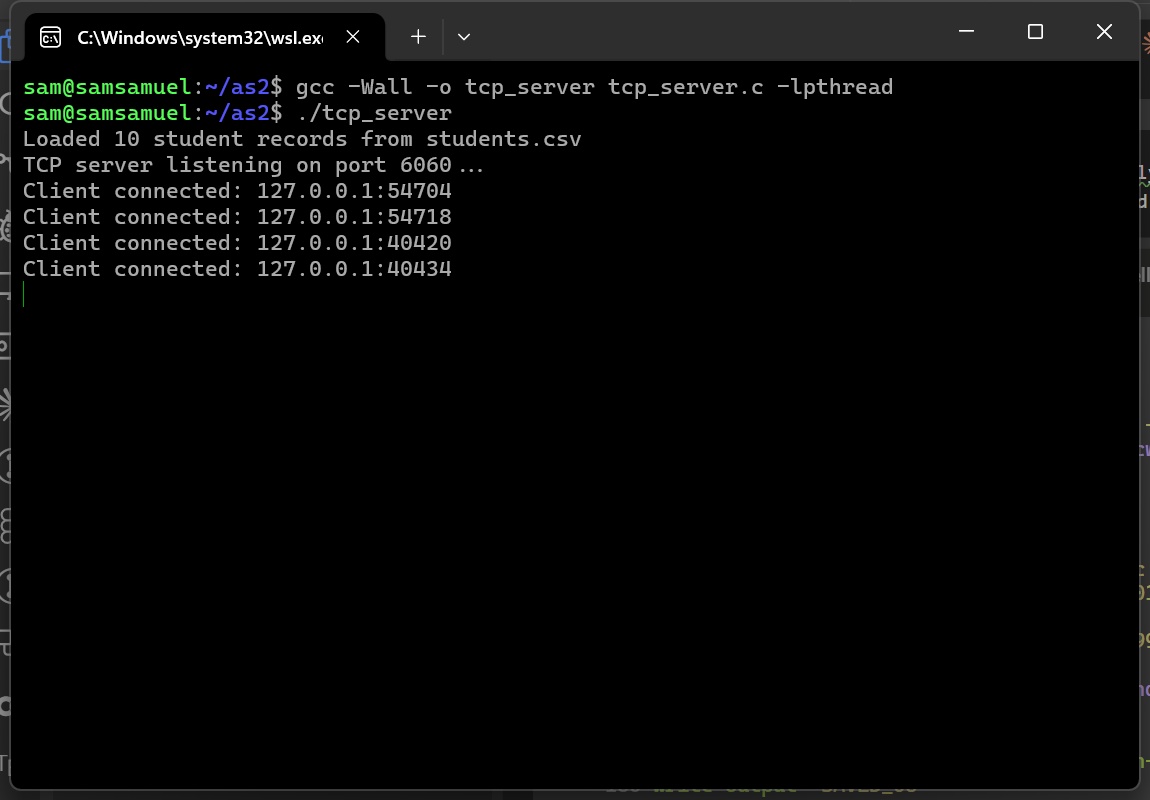
\includegraphics[width=0.85\linewidth]{ss/01_tcp_server.png}
\caption{TCP server terminal, accumulated log: a found lookup, a not-found lookup, and two
near-simultaneous client connections handled by separate threads.}
\end{figure}

\begin{figure}[H]
\centering
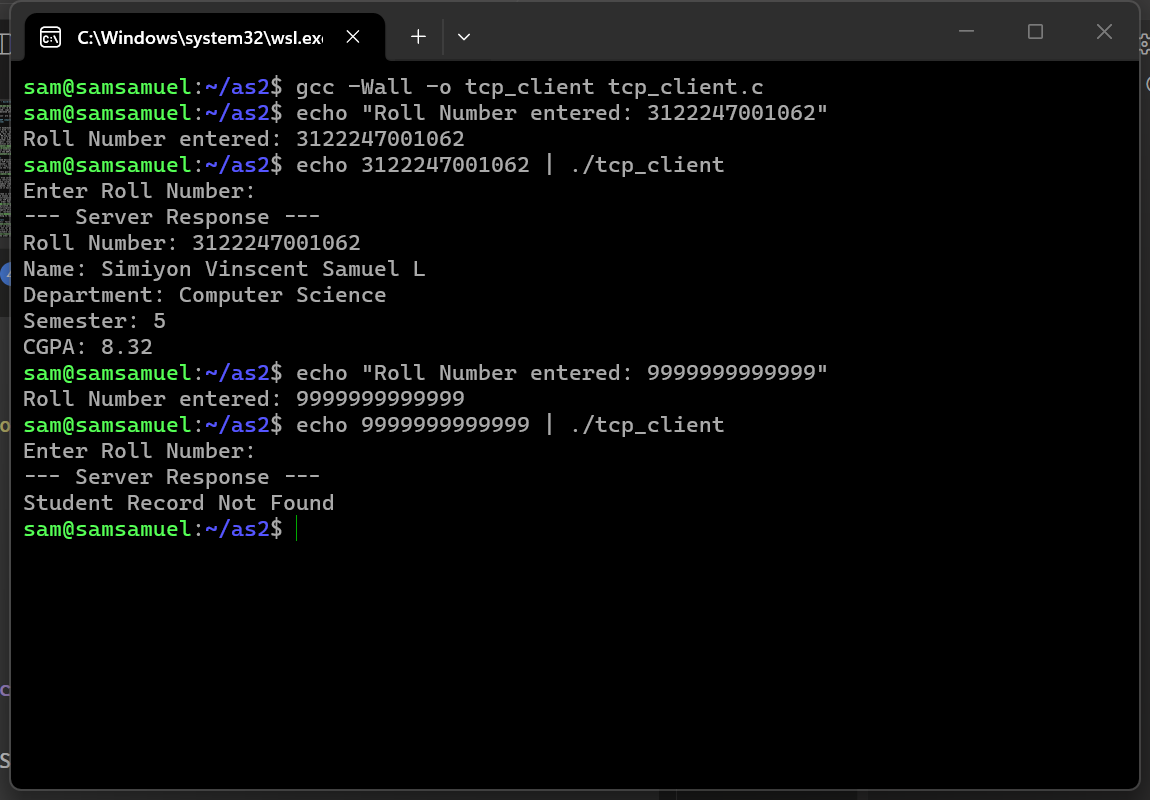
\includegraphics[width=0.85\linewidth]{ss/02_tcp_client_found_notfound.png}
\caption{TCP client run twice in sequence -- first an existing roll number returning the
full profile, then a roll number not in students.csv.}
\end{figure}

\begin{figure}[H]
\centering
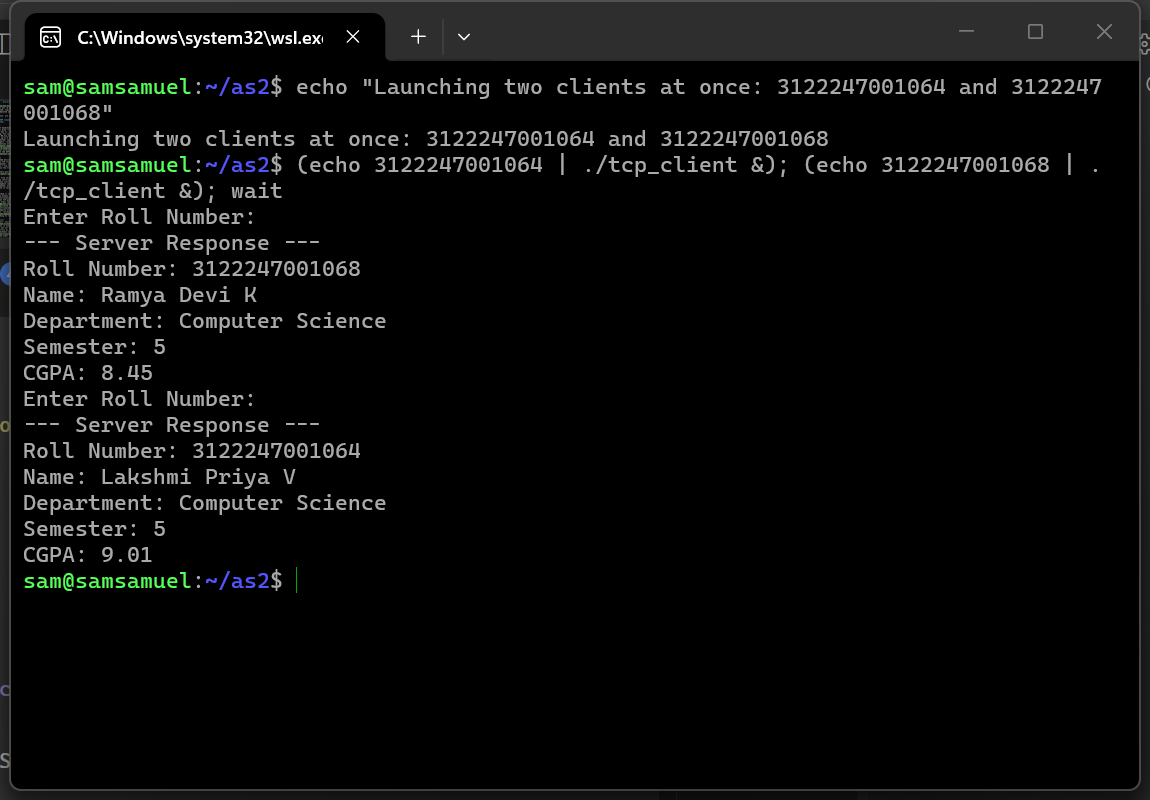
\includegraphics[width=0.85\linewidth]{ss/03_tcp_concurrent.png}
\caption{Two tcp\_client processes launched together against the same running server; both
receive their own correct reply, proving the pthread concurrency actually works.}
\end{figure}

\section*{Part 1(b): UDP Client--Server -- Verify Student Record}
\texttt{udp\_server.c} listens on port 6061 but never calls \texttt{listen()} or
\texttt{accept()} -- there is no connection to accept, just a single
\texttt{recvfrom()}/\texttt{sendto()} loop handling one datagram at a time. Because the
whole exchange fits in one loop iteration and the reply is intentionally tiny (roll
number and name only, per the 1(b) spec), one thread is enough; there is no per-client
state to hand off anywhere.

\begin{lstlisting}[caption={Excerpt of udp\_server.c -- the main recvfrom()/sendto() loop}]
while (1) {
    int n = recvfrom(sock, buf, sizeof(buf) - 1, 0,
                      (struct sockaddr *)&client_addr, &client_len);
    if (n <= 0) continue;
    buf[n] = '\0';
    buf[strcspn(buf, "\r\n")] = '\0';

    char response[BUF_SIZE];
    int found = 0;

    for (int i = 0; i < student_count; i++) {
        if (strcmp(students[i].roll, buf) == 0) {
            snprintf(response, sizeof(response), "Roll Number: %s\nName: %s\n",
                     students[i].roll, students[i].name);
            found = 1;
            break;
        }
    }

    if (!found) {
        snprintf(response, sizeof(response), "Student Record Not Found\n");
    }

    sendto(sock, response, strlen(response), 0,
           (struct sockaddr *)&client_addr, client_len);
}
\end{lstlisting}

\begin{figure}[H]
\centering
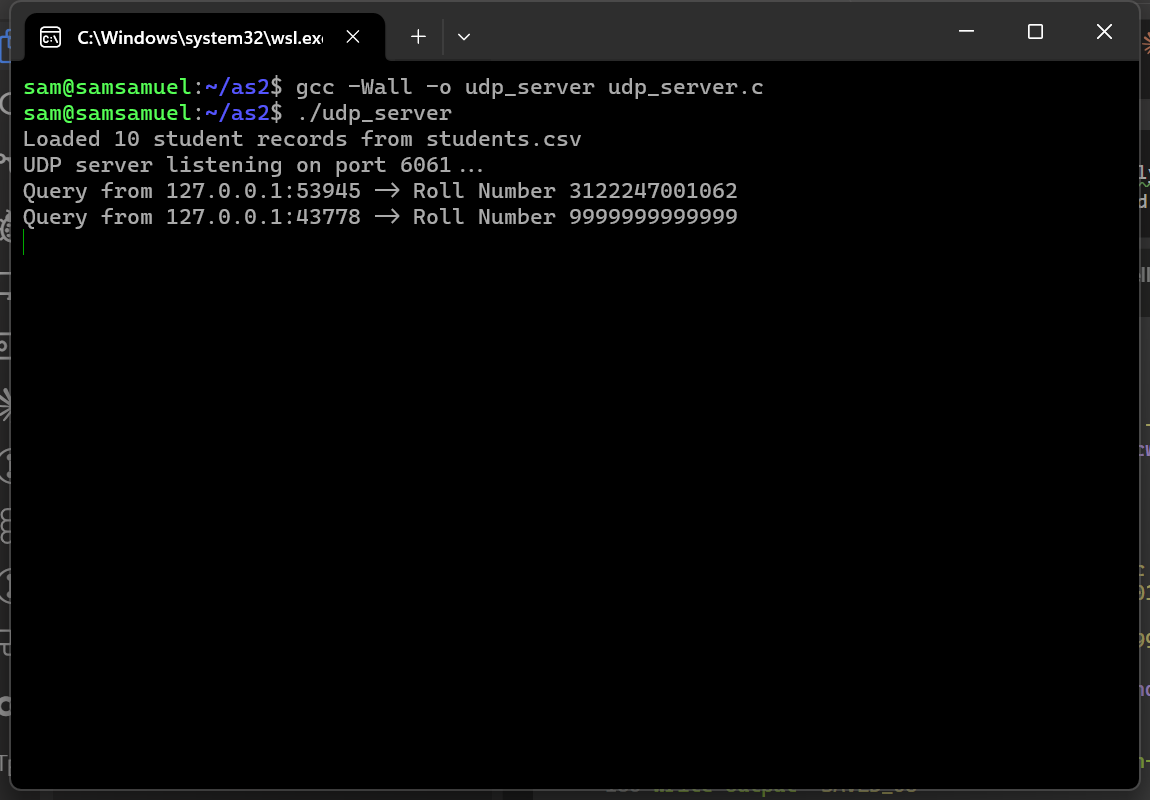
\includegraphics[width=0.85\linewidth]{ss/04_udp_server.png}
\caption{UDP server terminal log, showing incoming roll-number queries as they arrive.}
\end{figure}

\begin{figure}[H]
\centering
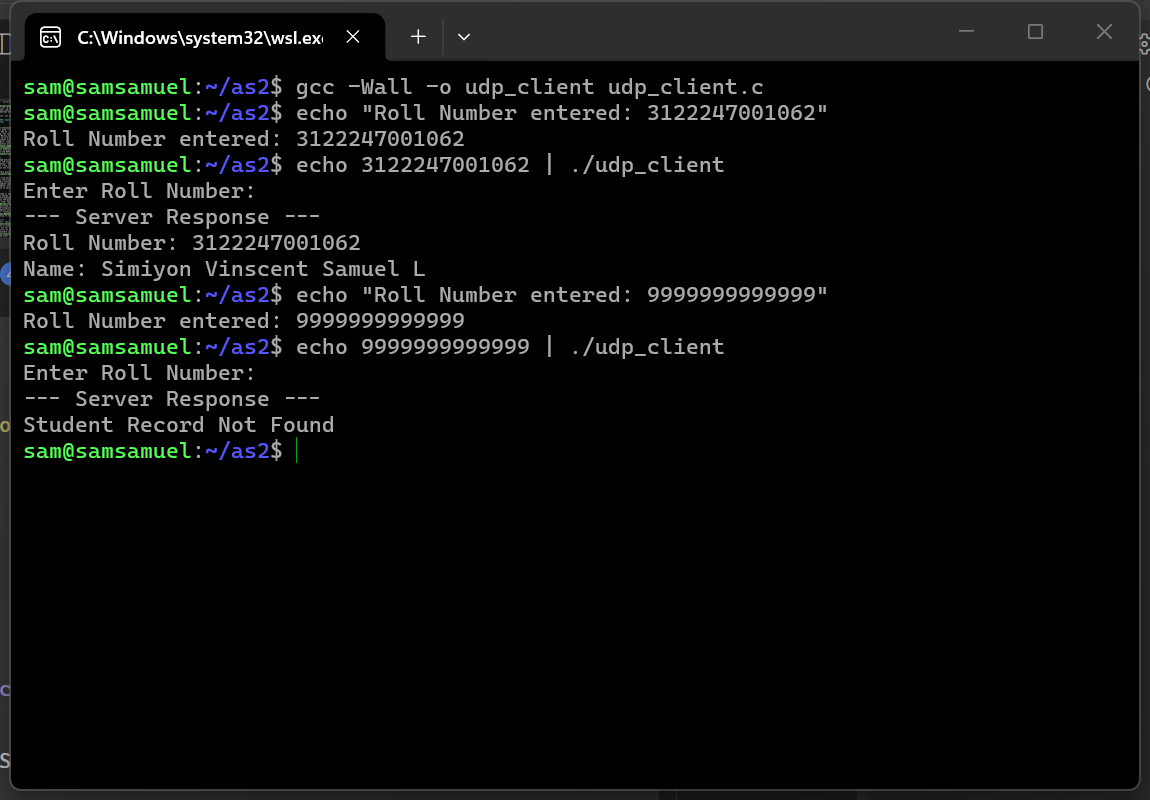
\includegraphics[width=0.85\linewidth]{ss/05_udp_client.png}
\caption{UDP client run twice -- an existing roll number returning just Roll Number and
Name, then a roll number not in students.csv.}
\end{figure}

\section*{Part 1c: TCP vs UDP Comparison}
\begin{table}[H]
\centering
\begin{tabular}{@{}p{2.6cm}p{5.6cm}p{5.6cm}@{}}
\toprule
\textbf{Aspect} & \textbf{TCP (Part 1a)} & \textbf{UDP (Part 1b)} \\
\midrule
Connection &
Explicit: \texttt{socket $\to$ bind $\to$ listen $\to$ accept} on the server,
\texttt{connect()} on the client. Each client shows up as a distinct ``Client connected''
line in the server log. &
None. \texttt{udp\_server} just \texttt{bind()}s and waits; the client fires one
\texttt{sendto()} with no setup step, and there is nothing like ``Client connected'' in
its log. \\
\addlinespace
Reliability &
Guaranteed by the kernel's TCP stack -- every request in testing got an answer, and
neither program has to handle a lost packet because the transport already does. &
No guarantee at all. \texttt{udp\_client.c} calls \texttt{recvfrom()} once and just
prints ``No response from server.'' if nothing comes back -- no retry, no timeout. \\
\addlinespace
Ordering &
Byte stream is ordered by the protocol (moot here since each exchange is one
request/response on a fresh connection, but true in general). &
Datagrams can in principle arrive out of order or duplicated; irrelevant for a
single-request-single-reply exchange but a real property of the protocol. \\
\addlinespace
Error Recovery &
\texttt{connect()} fails loudly and immediately if the server is not listening
(\texttt{perror} + exit) -- easy to detect and debug. &
\texttt{sendto()} ``succeeds'' even if nobody is listening; the client only finds out
indirectly when \texttt{recvfrom()} never returns. With no timeout coded here, an
unreachable server would hang the client. \\
\addlinespace
Communication &
Stream-oriented, connection-scoped, one pthread per client -- proven genuinely
concurrent in Figure~3, not just serialized by accident. &
Message-oriented, one \texttt{sendto}/\texttt{recvfrom} pair per exchange, stateless --
a single thread in a loop is enough since there is no connection to hand off. \\
\bottomrule
\end{tabular}
\end{table}

TCP is heavier (handshake, per-client thread, connection state) but guarantees the client
gets a correct, in-order, complete profile every time. UDP is lighter and faster for the
one-shot ``just confirm this roll number is valid'' case in 1(b), at the cost of no
delivery guarantee -- an acceptable trade here since it is a verify-only lookup, not a
full profile fetch.

\section*{Learning Outcome}
\begin{itemize}
\item Got a TCP server with a real pthread-per-client design working, and actually proved
the concurrency by hitting it with two clients at once instead of just assuming it from
the code.
\item Saw how much simpler a UDP server is to write -- no accept/connect, no per-client
thread -- but also how little protection that gives you: nothing in this lab's code would
even notice if a datagram went missing.
\item Parsing a CSV by hand with \texttt{fgets()}/\texttt{strtok()} was fiddlier than
expected (trailing newlines, the header row eating a real record if you forget to skip
it) -- a good reminder that ``just read the file'' is rarely as trivial as it sounds.
\end{itemize}

\end{document}
